\chapter{Experimentación y Resultados}
    Aquí se presentaran los resultados del \textbf{Análisis a Priori y Posteriori} del algoritmo de LCS.
    
\section{Algoritmo: LCS}
El algoritmo fue ejecutado en el lenguaje de programación \textbf{Python} en un entorno de \textbf{Linux}. A continuación se muestra el análisis de priori y posteriori. 
    \subsection{Análisis a Priori}
        La figura \ref{fig:priori} presenta el análisis a priori realizado sobre el pseudocódigo del algoritmo de LCS. Concluyendo que el algoritmo presenta \(T(n) = \theta(n*m)\) simplificando a \(\theta(n^{2})\)
        %\(f(n) = O(n)\)
        
        \begin{figure}[htp!]
            \centering
            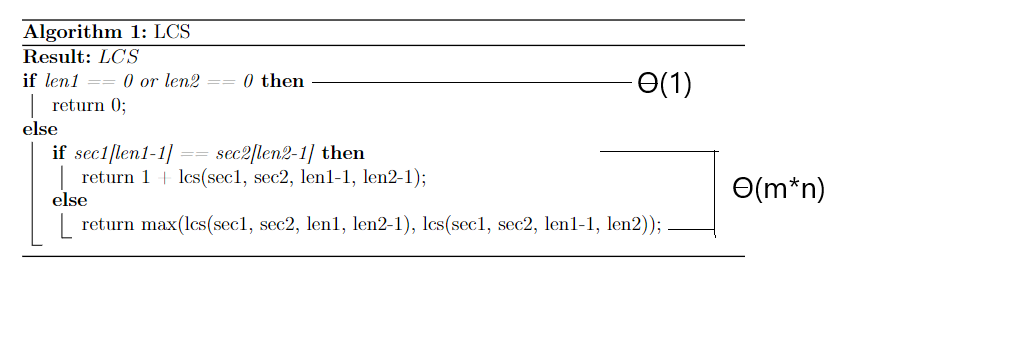
\includegraphics[width=1 \textwidth]{Images/A_Priori/priori.png}
            \caption{Análisis a Priori: LCS}
            \label{fig:priori}
        \end{figure}
    
    \newpage    
    \subsection{Análisis a Posteriori}
        En el análisis posteriori se verifica que el análisis a priori demostró que la complejidad del peor caso es \(T(n) = \theta(n^{2})\) dando un poco más la complejidad. En la figura \ref{fig:posteriori1} se muestra que el análisis a priori tuvo problemas al momento de ser planteado ya que la complejidad varió mínimamente. 
        \begin{figure}[htp!]
            \centering
            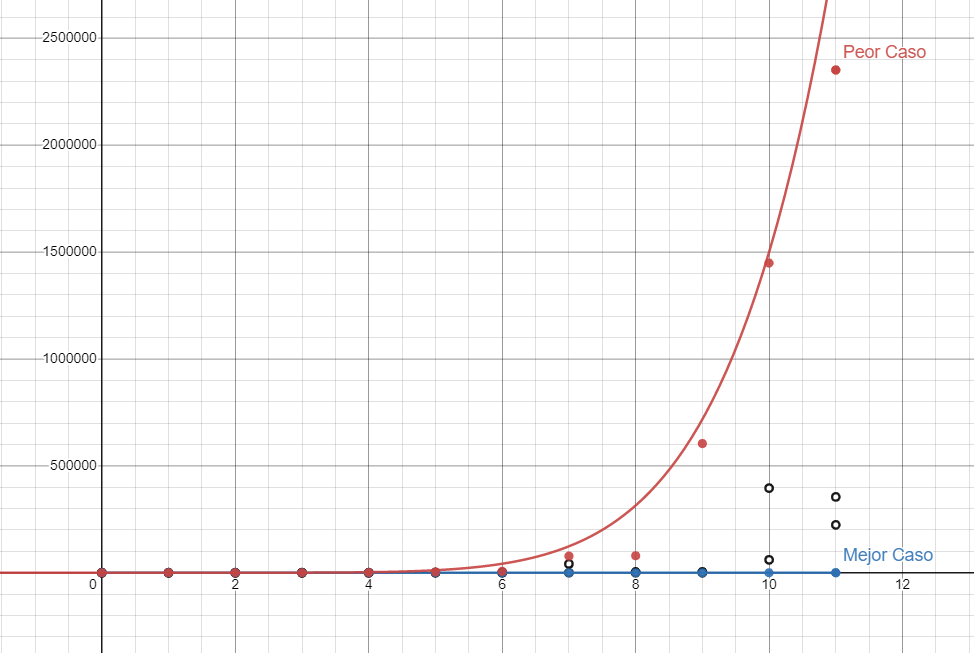
\includegraphics[width=1 \textwidth]{Images/A_Posteriori/posteriori.png}  
            \caption{Análisis a Posteriori: LCS}
            \label{fig:posteriori1}
        \end{figure}
    
    
    
    \newpage
    \section{Pantallas de Ejecución del Algoritmo}
    Se muestra en la figura \ref{fig:terminal} la ejecución del algoritmo, demostrando la velocidad del algoritmo.
    
        \begin{figure}[htp!]
            \centering
            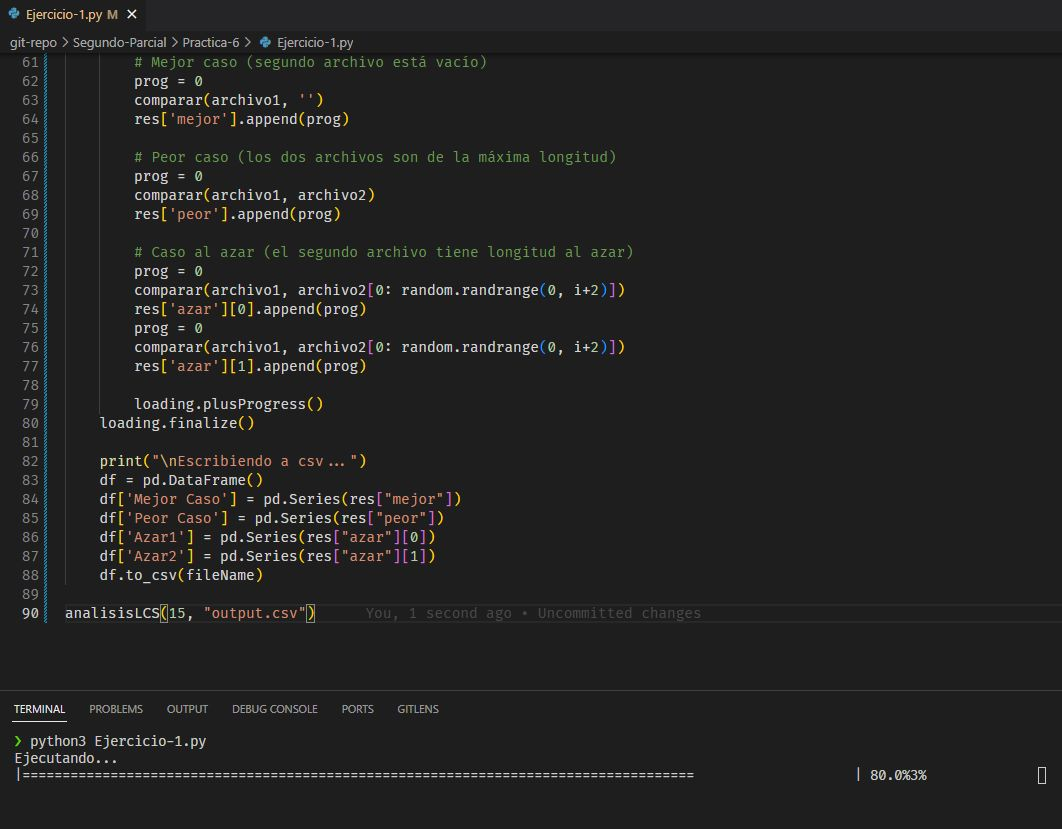
\includegraphics[width=0.8 \textwidth]{Images/Pantallas/ejecucion.jpg}  
            \caption{Ejecución de LCS}
            \label{fig:terminal}
        \end{figure}
    